\documentclass[12pt]{article}

\usepackage{sbc-template}

\usepackage{graphicx,url}
 
\usepackage[utf8]{inputenc}  

\usepackage{algorithm}
\usepackage{algpseudocode}
     
\sloppy

\title{H-FedChain: Uma Arquitetura Hierárquica Edge–Fog–Cloud com Consenso Baseado em Blockchain para Federated Learning Seguro em IoHT}

\author{Adriano Zavareze Righi\inst{1} }

\address{Mestrado em Computação Aplicada\\
Universidade Do Vale Do Rio Dos Sinos (UNISINOS)\\
   São Leopoldo -- RS -- Brasil
  \email{\ contato@adrianorighi.com}
}

\begin{document} 

\maketitle

\begin{abstract}
  The text follows the style of argumentative dissertation, containing two pages and     four paragraphs that are divided in: Introduction, first case, second case andvconclusion. The text model used was made available in the official domain of SBC (Sociedade Brasileira de Computação). The purpose of the text is to inform the author's opinion on two situations cited in Michael J. Sandel's book, "Justice -       What it is to do a certain thing", and explain its reasons.
\end{abstract}
     
\begin{resumo} 
  O texto segue o estilo de dissertação argumentativa, contendo duas páginas e quatro   parágrafos que se dividem em introdução, primeiro caso, segundo caso e conclusão. O modelo de texto utilizado foi o disponibilizado no domínio oficial  da SBC(Sociedade Brasileira de Computação). O objetivo do texto é informar a  opinião do autor sobre duas situações citadas no livro “Justiça - o que   é fazer a coisa certa” de Michael J. Sandel, e explicar seus motivos.
\end{resumo}


\section{Introdução}

WIP

\section{Conceitos Fundamentais}

\subsection{Internet of Health Things (IoHT)}

\subsection{Federated Learning (FL)}

\subsection{Blockchain}

\subsection{Mecanismos de consenso em Blockchain}

\subsection{Integração Blockchain e Federated Learning em IoHT}

\section{Trabalhos Relacionados}

Essa seção apresenta uma revisão crítica e estruturada da literatura científica sobre mecanismos de consenso em arquiteturas de aprendizado federado distribuído para saúde no contexto de cidades inteligentes (IoMT/IoHT). A revisão está organizada em subseções que contextualizam o estado da arte, agrupam as abordagens metodológicas identificadas, analisam criticamente convergências, divergências, lacunas e fragilidades, e posicionam a contribuição do presente trabalho.

\subsection{Estratégia de Busca}

A estratégia de busca foi definida com o objetivo de identificar estudos que integrem aprendizado federado, blockchain e mecanismos de consenso em arquiteturas distribuídas de saúde em ambientes edge–fog–cloud. As subseções a seguir descrevem as strings de busca adotadas, os filtros aplicados e os critérios de inclusão e exclusão utilizados.

\subsubsection{Strings de Busca Utilizadas}

As seguintes combinações booleanas foram utilizadas nas bases acadêmicas:

\begin{enumerate}
    \item \texttt{"blockchain" AND "federated learning" AND "healthcare" AND ("IoT" OR "IoMT") AND ("edge" OR "fog") AND "consensus protocol"}
    \item \texttt{"federated learning" AND ("edge" OR "fog" OR "cloud") AND "blockchain" AND ("IoMT" OR "IoHT") AND "smart cities"}
    \item \texttt{"consensus protocol" AND "blockchain" AND "distributed machine learning" AND "healthcare"}
    \item \texttt{"consensus" AND "blockchain" AND ("IoT" OR "healthcare") AND "edge computing"}
    \item \texttt{"FedAvg" AND "federated learning" AND "aggregation" AND "edge" AND "privacy" AND "healthcare"}
    \item \texttt{"permissioned blockchain" AND "Hyperledger Fabric" AND "healthcare" AND ("IoT" OR "privacy")}
    \item \texttt{"FedHealthFog" OR "FedBChain" OR "FL-Block" AND "healthcare" AND "fog" AND "blockchain"}
    \item \texttt{"lightweight consensus" AND "blockchain" AND "IoT" AND ("fog" OR "edge") AND "healthcare"}
\end{enumerate}

\subsubsection{Filtros Aplicados}

Para restringir a busca a estudos recentes e alinhados ao escopo deste trabalho, foram aplicados os filtros sintetizados na Tabela \ref{tab:filtros_busca} a seguir.

\begin{table}[!htbp]
\centering
\caption{Filtros aplicados na estratégia de busca}
\label{tab:filtros_busca}
\begin{tabular}{p{4cm}p{10cm}}
\toprule
\textbf{Critério} & \textbf{Parâmetro} \\
\midrule
\textbf{Período} & 2020--2026 \\
\midrule
\textbf{Tipo de publicação} & Artigos revisados por pares com DOI válido \\
\midrule
\textbf{Idioma} & Inglês ou Português \\
\midrule
\textbf{Área} & Computer Science, Medical Informatics, IoT, Distributed Systems \\
\midrule
\textbf{Bases consultadas} & IEEE Xplore, Elsevier ScienceDirect, JMIR, ACM Digital Library, Google Scholar \\
\bottomrule
\end{tabular}
\end{table}

\subsubsection{Critérios de Seleção}

Os critérios obrigatórios de inclusão adotados foram:

\begin{itemize}
    \item DOI válido e verificável;
    \item Publicados preferencialmente nos últimos seis anos (2020--2026), com exceção justificada para trabalhos seminais anteriores a esse período;
    \item Relevância direta ao tema: integração entre Aprendizado Federado, blockchain, protocolo de consenso e arquitetura edge-fog-cloud em contextos de IoMT/IoHT ou cidades inteligentes.
\end{itemize}

Os critérios de exclusão foram:

\begin{itemize}
    \item Trabalhos que não possuem as palavras chave no resumo ou introdução;
    \item Artigos que tratam de apenas um dos elementos da interseção temática, como por exemplo, somente blockchain sem FL, ou somente FL sem contexto distribuído;
    \item Publicações em idiomas distintos do inglês e português;
    \item Trabalhos duplicados.
\end{itemize}

\subsection{Contextualização do estado da Arte}

O paradigma atual da Internet das Coisas Médicas (IoMT) e da Internet das Coisas em Saúde (IoHT) evidencia uma migração de arquiteturas puramente centralizadas na nuvem para modelos distribuídos em camadas (\textit{edge–fog–cloud}), com o objetivo de reduzir latência, aliviar gargalos de comunicação e mitigar riscos de um ponto único de falha \cite{rajagopal2025,tripathy2024,ahmad2023}. Em cenários de monitoramento contínuo de pacientes, essa transição é particularmente relevante, pois a nuvem isoladamente tende a ser incapaz de processar, com latência ultra baixa, fluxos massivos de dados oriundos de sensores vestíveis e dispositivos IoMT \cite{rajagopal2025,tripathy2024,baucas2023}. Trabalhos como os de \cite{rajagopal2025,tripathy2024} demonstram que arquiteturas em três camadas, nas quais a borda realiza a coleta e pré-processamento, a \textit{fog} concentra agregações e filtragens intermediárias, e a nuvem mantém o histórico de longo prazo, reduzem significativamente o atraso e o uso da rede em comparação a abordagens totalmente centralizadas. Em geral, essas avaliações são conduzidas em cenários com número moderado de dispositivos e clientes, suficientes para observar tendências de desempenho, mas ainda aquém da densidade de nós esperada em IoMT urbana de larga escala \cite{rajagopal2025,tripathy2024,baucas2023}.

Paralelamente, a tecnologia \textit{blockchain} vem sendo incorporada como plano de confiança para garantir integridade, rastreabilidade e imutabilidade de dados e modelos em sistemas de saúde distribuídos \cite{ahmad2023,kamruzzaman2022,alam2022,baucas2023}. No lugar de atuar apenas como um repositório seguro, a \textit{blockchain} passa a coordenar o fluxo de informações entre dispositivos, camadas intermediárias e infraestrutura em nuvem, registrando transações médicas, atualizações de modelos de aprendizado e decisões de roteamento \cite{ahmad2023,alam2022,baucas2023}. \cite{ahmad2023} exemplificam esse papel ao propor uma arquitetura em que a camada fog é dividida em clusters críticos e não críticos, utilizando a \textit{blockchain} para registrar (minerar?) dados não críticos na nuvem, reduzindo custos operacionais sem comprometer a privacidade. De maneira complementar, \cite{kamruzzaman2022,alam2022} discutem arquiteturas conceituais que integram fog, IoMT e \textit{blockchain} para reforçar a interoperabilidade e a segurança em serviços de saúde para cidades inteligentes, ainda que sem validações em redes de grande escala.

No contexto específico de aprendizado federado, emergem propostas que combinam essa forma de aprendizado distribuído com \textit{blockchain} em arquiteturas \textit{edge–fog–cloud} voltadas à saúde \cite{rajagopal2025,ren2024,baucas2023,tripathy2024}. \cite{rajagopal2025} apresentam o framework FedSDM, no qual dados de ECG são processados em uma arquitetura de três camadas, empregando FedAvg para o treinamento federado e contratos inteligentes em uma \textit{blockchain} privada para registrar e coordenar as atualizações dos modelos locais, resultando em reduções expressivas de latência e uso de rede em comparação com soluções centradas apenas na nuvem. \cite{ren2024} propõem a arquitetura FLCoin, que utiliza uma \textit{blockchain} em duas camadas e um esquema de consenso por comitês, eleito de forma compatível com o cenário de aprendizado federado, a fim de diminuir o \textit{overhead} de comunicação e o tempo de treinamento, viabilizando maior escalabilidade em ambientes de borda. \cite{baucas2023} exploram a combinação de aprendizado federado com uma \textit{blockchain} privada em uma plataforma Fog-IoT para dispositivos vestíveis, demonstrando que a agregação em nós fog permite preservar a privacidade dos dados sensíveis e atenuar a heterogeneidade dos dispositivos na consolidação do modelo global. Já \cite{tripathy2024} focam a camada fog como orquestradora das agregações federadas, elegendo dinamicamente nós de névoa como agregadores globais com base em carga de trabalho e atraso, o que reduz o tempo médio de comunicação em comparação a abordagens que utilizam apenas a nuvem, ainda em cenários com número limitado de clientes.

Um aspecto central nos trabalhos que combinam aprendizado federado e blockchain, é o tratamento de segurança e privacidade em cenários de saúde \cite{rajagopal2025,baucas2023,ahmad2023}. Ao manter os dados clínicos sensíveis na edge e na fog e compartilhar apenas parâmetros de modelos ou estatísticas agregadas, o aprendizado federado reduz a necessidade de transferência de grandes volumes de dados entre camadas, mitigando riscos de exposição e vazamento de informações \cite{rajagopal2025,tripathy2024,baucas2023}. A blockchain, por sua vez, fornece um registro imutável das atualizações de modelos, transações e decisões de roteamento, o que reforça a auditabilidade e a rastreabilidade das operações, complementando os mecanismos tradicionais de privacidade e controle de acesso descritos em arquiteturas baseadas em fog e IoMT \cite{ahmad2023,kamruzzaman2022,alam2022}.

Entretanto, a simples combinação de aprendizado federado e \textit{blockchain} não é suficiente para garantir desempenho e escalabilidade em contextos IoMT. Protocolos de consenso tradicionais, como o \textit{Proof of Work} (PoW), revelam-se energeticamente inviáveis e inadequados em termos de latência para dispositivos médicos com recursos limitados e para camadas fog sujeitas a variações dinâmicas de carga \cite{laouamri2025,aljoboury2020}. \cite{laouamri2025} propõem uma abordagem baseada em topologia fog e um protocolo de consenso leve, denominado RaftNode, com assinaturas Schnorr, buscando otimizar o consumo de energia e manter alta vazão na rede em cenários de saúde distribuídos, ainda que em simulações com tamanho de rede controlado. \cite{aljoboury2020}, por sua vez, avaliam empiricamente PoW, \textit{Proof of Stake} (PoS) e PBFT em uma arquitetura de \textit{Blockchain of Things} hospedada em servidores fog, identificando que o PoS apresenta menor latência e menor consumo de recursos computacionais do que PoW e PBFT em ambientes fog emulados.

Além das comparações entre protocolos já consolidados, surgem propostas que buscam tornar o consenso mais adaptativo e alinhado às características dinâmicas de redes IoMT \cite{cheikhrouhou2023,murthy2026,ren2024}. \cite{cheikhrouhou2023} apresentam um sistema de monitoramento remoto de pacientes alicerçado em uma \textit{blockchain} leve operando em três camadas, no qual o consenso é concebido para reduzir a complexidade computacional e atender às restrições de latência na edge e na fog. \cite{murthy2026} introduzem um framework adaptativo para IoMT federado em Hyperledger Fabric, com um protocolo de consenso baseado em aprendizado por reforço (ABFT-RL) que ajusta dinamicamente parâmetros como \textit{timeout} e tamanho de bloco, obtendo melhorias de vazão e latência em comparação com versões clássicas de PBFT e Raft. \cite{ren2024} também exploram consensos orientados a comitês em sua arquitetura FLCoin, aproximando a lógica de consenso das próprias dinâmicas do aprendizado federado.

Em resumo, os trabalhos analisados convergem na utilização de arquiteturas em múltiplas camadas (\textit{edge–fog–cloud}) e na adoção de \textit{blockchain} como plano de confiança para aplicações de saúde em ambientes IoMT, incorporando, em alguns casos, aprendizado federado para preservar a privacidade dos dados na edge \cite{rajagopal2025,tripathy2024,ahmad2023,kamruzzaman2022,alam2022,ren2024,baucas2023}. No entanto, apesar de existirem propostas de protocolos de consenso leves, comparações entre esquemas clássicos e tentativas de consenso adaptativo, ainda é limitada a quantidade de soluções que articulam de forma integrada: (i) os requisitos de latência e energia típicos da IoMT, (ii) a natureza hierárquica edge–fog–cloud, (iii) as particularidades da agregação de modelos em aprendizado federado e (iv) o uso do consenso como mecanismo explícito de auditoria das contribuições dos nós no contexto de cidades inteligentes \cite{laouamri2025,cheikhrouhou2023,murthy2026,aljoboury2020,rajagopal2025,ren2024,baucas2023}. Essa lacuna demonstra a necessidade de arquiteturas de consenso em \textit{blockchain} explicitamente projetadas para o suporte a aprendizado federado em cenários de saúde urbanos, tanto em termos funcionais quanto em termos de escala de rede, o que motiva a proposta desenvolvida nesse trabalho.

A Tabela \ref{tab:comparativa} sintetiza as principais características dos trabalhos analisados, destacando os contextos de avaliação e as lacunas identificadas, que fundamentam essa investigação.

\begin{table}[h!]
    \centering
    \caption{Consolidação da literatura: Técnicas, Métricas e Gaps.}
    \label{tab:comparativa}
    \small
    \begin{tabular}{|p{2.5cm}|p{2.5cm}|p{2.8cm}|p{2.5cm}|p{2.5cm}|}
        \hline
        \textbf{Autor/Ano} & \textbf{Técnica Principal} & \textbf{Dataset/Contexto} & \textbf{Métrica} & \textbf{Gap Identificado} \\ \hline
        Rajagopal (2025) & FedSDM (FL + Ganache BC) & EUA Dataset (ECG - 5.000 leituras) & Latência (-79\%) & Falta de testes em implantação real. \\ \hline
        Cheikhrouhou (2023) & BC Leve + Fog Inteligente & Sintético (RPM - 24 máquinas ECG) & Responsividade (+40\%) & Agendamento de dados injusto no Fog. \\ \hline
        Laouamri (2025) & RaftNode + Schnorr & Simulação NS3 (30 sensores, 8Mb dados) & Throughput / Energia & Requisito de altos recursos de simulação. \\ \hline
        Murthy (2026) & ABFT-RL (Consenso via IA) & Icentia 11k / Fitbit (10M registros/1M transações)& Throughput (+43\%) & Heterogeneidade real não capturada. \\ \hline
        Ren (2024) & FLCoin (BC de 2 camadas) & MNIST / Edge Nodes (70.000 imagens) & Overhead Comm (-90\%) & Segurança em janelas de comitê rotativas. \\ \hline
        Tripathy (2024) & FedHealthFog (Heurística Greedy) & PhysioNet (Sinais Simulados 5-20 clientes) & Delay (-87\%) & Ausência de segurança intrínseca no consenso. \\ \hline
        Ahmad (2023) & Clusters CFC/NFC & Sinais Vitais (1.200 características) & Acurácia (99\%) & Latência de mineração na nuvem. \\ \hline
        Kamruzzaman (2022) & SLR (PRISMA) & 10 artigos seminais / Smart Cities & Interoperabilidade & Escassez de estudos integradores (3 camadas). \\ \hline
        Alam (2022) & Framework BFCM & Revisão IoMT & Confiabilidade & Falta de implementação experimental. \\ \hline
        Baucas (2023) & Fog-IoT Platform & HAR UCI (10.299 instâncias) & Integridade / Privacidade & Escalabilidade para redes massivas. \\ \hline
        Al-Joboury (2020) & BoT (Fog Server) & Linux-based Fog (Stream simulado 100 dados/seg) & CPU / Memória & Foco em emulação local/virtual. \\ \hline
    \end{tabular}
\end{table}

\subsubsection*{Análise Crítica}

A partir da síntese apresentada, é possível identificar alguns padrões recorrentes e lacunas relevantes na literatura recente sobre IoMT/IoHT, aprendizado federado, blockchain e protocolos de consenso em ambientes distribuídos de saúde \cite{rajagopal2025,cheikhrouhou2023,laouamri2025,murthy2026,ren2024,tripathy2024,ahmad2023,kamruzzaman2022,alam2022,baucas2023,aljoboury2020}. Em primeiro lugar, observa-se uma convergência em direção a arquiteturas hierárquicas em múltiplas camadas, nas quais dispositivos de borda realizam coleta e pré-processamento, a névoa concentra agregações e filtragens intermediárias, e a nuvem mantém dados históricos e capacidades analíticas de maior porte \cite{rajagopal2025,tripathy2024,ahmad2023,kamruzzaman2022,alam2022}. Essa organização edge–fog–cloud se mostra eficaz para reduzir latência e tráfego em comparação com soluções estritamente centralizadas, mas raramente é acompanhada de um desenho de consenso explicitamente otimizado para o contexto federado de IoMT/IoHT, especialmente quando se considera a densidade de dispositivos e a variabilidade de carga típica de cidades inteligentes.

Em segundo lugar, embora a blockchain seja amplamente reconhecida como o plano de confiança adequado para assegurar integridade, auditabilidade e imutabilidade em sistemas de saúde distribuídos, a forma como o consenso é implementado ainda apresenta limitações importantes \cite{ahmad2023,kamruzzaman2022,alam2022,baucas2023}. Abordagens que empregam PoW ou variações de protocolos clássicos tendem a ser incompatíveis com as restrições de energia e processamento típicas de dispositivos médicos e nós de névoa, o que motivou o estudo de alternativas mais leves como RaftNode, PoS e consensos simplificados em arquiteturas fog \cite{laouamri2025,aljoboury2020,cheikhrouhou2023}. Trabalhos como os de Laouamri et al. e Al-Joboury e Al-Hemiary evidenciam que a adoção de protocolos mais leves pode reduzir consumo de recursos e latência na camada fog, porém a integração desses mecanismos à lógica de aprendizado federado ainda é incipiente, e as avaliações são realizadas, em sua maior parte, em ambientes simulados ou emulados com dimensões de rede limitadas \cite{laouamri2025,aljoboury2020}.

Em terceiro lugar, emergem propostas que aproximam o consenso dos próprios ciclos de aprendizado federado, seja por meio de comitês associados a participantes do FL, seja por algoritmos adaptativos ancorados em aprendizado por reforço. \cite{murthy2026,ren2024} Ren et al. introduzem a arquitetura FLCoin, na qual um esquema de consenso baseado em comitês busca otimizar a comunicação e o tempo de treinamento, reduzindo o overhead em ambientes de borda; entretanto, o mecanismo de comitê ainda não explora explicitamente características específicas da IoMT, como criticidade das leituras médicas ou mobilidade dos nós. \cite{ren2024} Murthy e Lawanya Shri propõem o ABFT-RL em Hyperledger Fabric, que ajusta dinamicamente parâmetros de consenso com base em métricas de desempenho de rede, obtendo ganhos de vazão e latência; contudo, o foco recai mais sobre a camada de nuvem/federação de serviços do que sobre a interação fina com dispositivos médicos em contextos edge–fog–cloud, além de exigir considerável capacidade de processamento para o agente de RL. \cite{murthy2026}

Por outro lado, trabalhos como os de Rajagopal et al., Tripathy et al. e Baucas et al. demonstram o potencial do aprendizado federado em aplicações de saúde, preservando a privacidade dos dados na borda e reduzindo custos de comunicação. \cite{rajagopal2025,tripathy2024,baucas2023} Rajagopal et al. integram FL e blockchain em uma arquitetura de três camadas, mas a lógica de consenso é tratada de forma relativamente genérica, sem detalhar critérios de validação específicos para atualizações de modelos. \cite{rajagopal2025} Tripathy et al. concentram-se em heurísticas de eleição de agregadores fog para reduzir atraso, sem acoplar essa dinâmica a um mecanismo de consenso em blockchain ou a regras formais de auditoria das contribuições dos nós. \cite{tripathy2024} Baucas et al. utilizam blockchain para assegurar integridade de atualizações de modelos, porém não investigam profundamente a adaptação do consenso às variações de carga, conectividade e heterogeneidade de dispositivos \textit{wearables} em cenários de larga escala. \cite{baucas2023}

Do ponto de vista de segurança e privacidade, os trabalhos analisados evidenciam que a combinação de aprendizado federado e blockchain oferece um caminho promissor para reduzir o compartilhamento de dados sensíveis entre dispositivos, fog e nuvem, ao mesmo tempo em que mantém trilhas de auditoria robustas para operações críticas \cite{rajagopal2025,baucas2023,ahmad2023}. No entanto, a maioria das propostas ainda trata essas propriedades de forma agregada, sem explorar em profundidade como o protocolo de consenso pode incorporar métricas de privacidade ou criticidade clínica na validação das atualizações de modelos e transações médicas \cite{cheikhrouhou2023,laouamri2025,murthy2026}. Em particular, poucos trabalhos definem explicitamente quais critérios são verificados pelo consenso para aceitar ou rejeitar atualizações de modelos (por exemplo, consistência estatística, contribuição marginal para a acurácia global, etc.), o que limita o uso da blockchain como auditoria completa do processo de aprendizado federado em redes IoMT/IoHT \cite{rajagopal2025,ren2024,baucas2023,murthy2026,aljoboury2020}.

Finalmente, estudos de natureza mais conceitual, como os de Kamruzzaman et al. e Alam et al., reforçam a pertinência de combinar fog computing, IoMT e blockchain para aplicações de saúde em cidades inteligentes, mas não avançam para a definição de um protocolo de consenso que considere simultaneamente requisitos de latência, energia, confiabilidade e dinâmica do aprendizado federado \cite{kamruzzaman2022,alam2022}. Esse panorama indica que, embora existam contribuições relevantes em cada um dos eixos (arquiteturas edge–fog–cloud, aprendizado federado em saúde, blockchain como plano de confiança e protocolos de consenso leves ou adaptativos), ainda é raro encontrar soluções que integrem de forma coesa todos esses elementos no contexto específico de IoMT/IoHT urbano.

Diante dessas observações, o presente trabalho se posiciona no espaço de interseção entre aprendizado federado, IoMT/IoHT e blockchain, com foco no desenho de um protocolo de consenso, diretamente no plano de controle da rede fog, adaptado às particularidades de ambientes de saúde em cidades inteligentes. Em termos gerais, busca-se conceber um mecanismo de consenso em blockchain capaz de: (i) operar de forma eficiente em arquiteturas hierárquicas edge–fog–cloud, (ii) considerar explicitamente as restrições de recursos e requisitos de latência típicos de dispositivos e gateways médicos, e (iii) alinhar-se ao ciclo de agregação de modelos do aprendizado federado, de forma a reduzir overhead de comunicação e aumentar a robustez frente à heterogeneidade e dinâmica da IoMT. A partir da análise crítica dos trabalhos, conclui-se que essa combinação ainda não foi plenamente explorada, o que evidencia uma lacuna concreta na literatura e fundamenta a relevância da arquitetura de consenso em blockchain proposta nesse trabalho para o suporte ao aprendizado federado em ambientes de IoMT/IoHT.

\section{Modelo H-FedChain}

A integração entre tecnologias de \textit{Federated Learning}~(FL) e infraestruturas de blockchain permissionada em ambientes distribuídos de saúde digital tem recebido crescente atenção da comunidade científica, principalmente diante das exigências de privacidade impostas pela LGPD (BR), HIPAA (USA) e GDPR (UE). Apesar dos avanços recentes, a literatura ainda apresenta lacunas na definição de arquiteturas capazes de integrar, de forma sistemática, o treinamento colaborativo distribuído, a rastreabilidade imutável e a verificação criptográfica \textit{end-to-end} em um único modelo operacional voltado para dispositivos de Internet das Coisas Médicas (IoMT).

Nesse trabalho é proposta a arquitetura \textbf{H-FedChain} (\textit{Hierarchical Federated Chain}), um modelo distribuído multicamadas desenvolvido para suportar treinamento federado com preservação de privacidade em ambientes IoMT. A visão geral da arquitetura proposta é apresentada na Figura~\ref{fig:hfedchain_architecture}.

\begin{figure}[ht!]
    \label{fig:hfedchain_architecture}
    \centering
    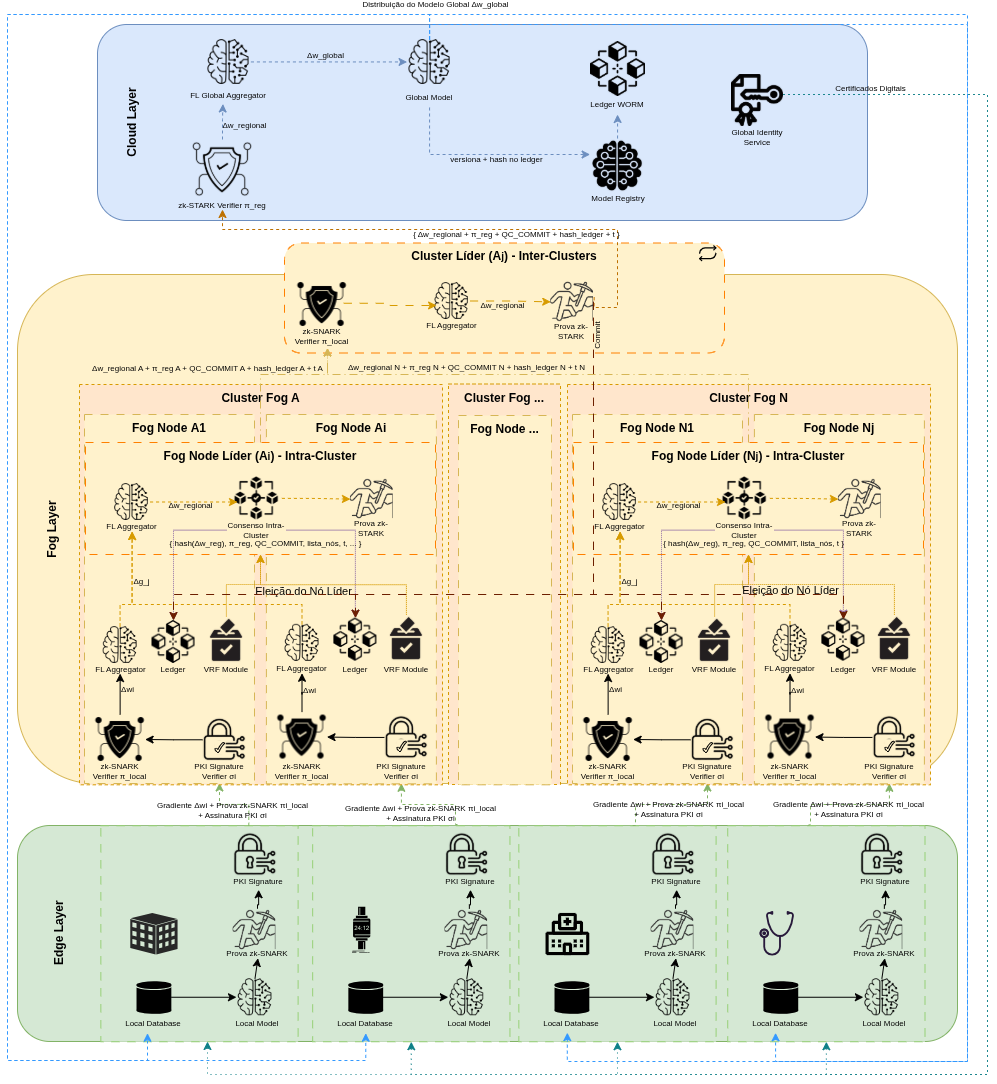
\includegraphics[width=\textwidth]{./images/H-FedChain-Architecture.png}
    \caption{Arquitetura hierárquica da H-FedChain e seus componentes distribuídos.}
\end{figure}

A arquitetura é estruturada sobre três pilares principais: (i)~organização \textbf{hierárquica} em camadas verticais com responsabilidades computacionais proporcionais; (ii)~uso de \textbf{Federated Learning} como mecanismo de treinamento sem compartilhamento de dados clínicos; e (iii)~adoção de \textbf{blockchain permissionada} com consenso distribuído tolerante a falhas como base para rastreabilidade e auditabilidade.

Essa seção está organizada da seguinte forma. A Subseção~\ref{sec:decisoes} apresenta as decisões de projeto e suas justificativas técnicas. A Subseção~\ref{sec:descricao} descreve os componentes arquiteturais e as camadas do sistema.

\subsection{Decisões de Projeto}
\label{sec:decisoes}

O projeto da H-FedChain é orientado por quatro restrições fundamentais do domínio de saúde digital:

\begin{enumerate}
  \item \textbf{Privacidade de dados clínicos}: dados de pacientes estão sujeitos a proteção legal obrigatória, exigindo que nenhum dado bruto seja transmitido para fora do dispositivo de origem;
  \item \textbf{Recursos restritos em dispositivos IoMT}: sensores e monitores médicos operam com severas limitações computacionais e energéticas, tornando inviável a execução de protocolos intensivos na camada periférica;
  \item \textbf{Participantes potencialmente desonestos}: dispositivos médicos e redes hospitalares são ambientes sujeitos a falhas, desconexões e comportamento potencialmente adversarial;
  \item \textbf{Auditabilidade regulatória}: legislações da área da saúde exigem trilhas de auditoria imutáveis para todo o ciclo de processamento de dados clínicos e modelos.
\end{enumerate}

A partir dessas restrições, foram estabelecidas as seguintes decisões de projeto.

\subsubsection{Separação Vertical em Camadas Hierárquicas}

A organização em três camadas verticais, Edge, Fog e Cloud, permite distribuir responsabilidades computacionais de forma proporcional à capacidade de cada nível, evitando tanto a sobrecarga dos dispositivos periféricos quanto a centralização excessiva na nuvem~~\cite{rajagopal2024leveraging,awaisi2025hybrid}. Essa organização permite escalar cada nível independentemente e limitar o impacto de falhas ao escopo da camada afetada.
A camada Fog é utilizada como intermediária para absorver grande parte da carga de validação e agregação, reduzindo latência e volume de dados transmitidos para a nuvem.
A camada Cloud possui papel propositalmente restrito à verificação e orquestração do sistema, não atuando como repositório de dados clínicos, em conformidade com o princípio de minimização de dados.

\subsubsection{Federated Learning como Paradigma de Treinamento}

O FL foi adotado como paradigma central por permitir a otimização colaborativa de um modelo global sem que os participantes tenham acesso aos dados privados uns dos outros, transmitindo apenas gradientes calculados localmente~\cite{nguyen2022federated,pfitzner2023flhealthcare}. A cada rodada $t$, cada dispositivo Edge recebe os pesos do modelo global $w^{(t)}$ e computa o gradiente local $\Delta w_i$ sobre sua base de dados clínica privada, sem transmitir nenhum dado bruto.

Entretanto, o FL clássico apresenta vulnerabilidade a ataques de \textit{gradient poisoning}, nos quais participantes maliciosos submetem atualizações adulteradas com o objetivo de comprometer o modelo global. Essa vulnerabilidade justifica a utilização de algoritmos de agregação robusta Multi-Krum~\cite{blanchard2017machine}, aplicados na camada Fog antes de qualquer confirmação de bloco, permitindo tolerar formalmente até $f < n/3$ participantes maliciosos entre $n$ contribuintes ~\cite{awaisi2025hybrid,rajagopal2025ai}.  O Multi-Krum seleciona os $m = n - f$ gradientes com menor soma de distâncias euclidianas mútias, onde $n$ é o número total de contribuintes e $f < n/3$ o limite de participantes maliciosos toleráveis, garantindo robustez formal contra ataques coordenados. A escolha do Multi-Krum em detrimento do Trimmed Mean, é motivada pela sua robustez superios em cenários \textit{non-IID} e contra ataques concentrados, condição frequente em redes hospitalares comprometidas.

\subsubsection{Blockchain Permissionada na Camada Fog}

A decisão de posicionar a blockchain na camada Fog, e não na Cloud como observado em trabalhos correlatos~\cite{wu2024scalable,rajagopal2024leveraging}, é motivada por três fatores:
(i)~\textbf{latência}, uma vez que a confirmação de blocos deve ocorrer próxima à origem dos dados para satisfazer os requisitos de tempo real de aplicações IoMT;
(ii)~\textbf{descentralização de confiança}, evitando ponto único de controle na nuvem; e
(iii)~\textbf{verificabilidade local}, permitindo que cada cluster mantenha auditoria independente sobre seu histórico de modelos regionais.

A utilização de blockchain permissionada em detrimento de blockchain pública é justificada pela possibilidade de controle de acesso baseado em identidade (PKI) e pela eliminação do elevado custo energético associado a mecanismos de consenso baseados em prova de trabalho, inadequados para nós Fog com recursos limitados~\cite{wu2024scalable}. Cada cluster Fog mantém seu próprio ledger replicado entre todos os Fog Nodes do cluster, garantindo que a integridade dos dados não dependa de um servidor central. A imutabilidade retroativa é assegurada pelo encadeamento de hashes: cada bloco registra o hash do bloco anterior, tornando qualquer adulteração computacionalmente inviável~\cite{qammar2023securing}.

\subsubsection{Protocolo de Consenso HotStuff BFT}

A H-FedChain adota o protocolo \textbf{HotStuff} como mecanismo de consenso distribuído tolerante a falhas Bizantinas (\textit{Byzantine Fault Tolerance}, BFT), operando em dois níveis: intra-cluster e inter-cluster (inter-regional). O HotStuff foi selecionado em detrimento do PBFT clássico por usa complexidade de mensagens $\mathcal{O}(n)$ por fase, em contraste com $\mathcal{O}(n^2)$ do PBFT, o que o torna escalável para clusters com dezenas de nós Fog.

O protocolo executa três fases sequenciais: \textbf{PREPARE}, \textbf{PRE-COMMIT} e \textbf{COMMIT}. Em cada fase, o líder coleta votos dos nós participantes e, ao atingir o quórum $\lceil 2n/3 \rceil + 1$, agrega as assinaturas em um \textit{Quorum Certificate} (QC), que serve como pré-requisito para a fase seguinte. O QC\_COMMIT, emitido ao final da fase COMMIT, é o gatilho que autoriza cada Ledger Peer a persistir o bloco em seu ledger local.

A tolerância a falhas garante operação correta na presença de até $f < n/3$ nós Bizantinos. Em caso de falha do líder, o protocolo executa automaticamente um \textit{view-change}, promovendo o próximo candidato eleito pelo mecanismo VRF, descrito na Seção~\ref{sec:vrf}, sem interromper a operação do cluster.

\subsubsection{Eleção de Líder por VRF}
\label{sec:vrf}

A eleição do líder de consenso em cada rodada é realizada por meio de uma \textbf{Função Aleatória Verifiável} (\textit{Verificable Random Function}, VRF) eliminando o papel de representante fixo e o consequente ponto único de falha (SPOF). O protocolo de eleição opera da seguinte forma:

\begin{enumerate}
\item \textbf{Semente compartilhada}: ao início da rodada $t$, todos os nós derivam determinísticamente a semente $s_t = {hash}(B_{t-1})$, onde $(B_{t-1})$ é o hash do último bloco confirmado no ledger do cluster;
\item \textbf{Cálculo local}: cada nó $j$ computa indepementemente o par 
\[
(y_j,\; \pi_j^{{vrf}}) \leftarrow {VRF.Eval}(sk_j,\; s_t),
\]
onde $sk_j$ é sua chave privada PKI, $y_j \in \{0,1\}^{256}$ é a saída pseudoaleatória e $\pi_j^{{vrf}}$ é a prova de corretude que permite a qualquer observador verificar que $y_j$ foi calculado corretamente. Em seguida, o nó difunde o triplo $(j,\; y_j,\; \pi_j^{{vrf}})$ para todos os pares do cluster;
\item \textbf{Seleção}: cada nó coleta os triplos dos demais participantes durante o intervalo ${TIMEOUT\_VRF}$ e forma o conjunto de candidatos válidos. O líder da rodada é determinado como:
\[
{L\'{\i}der}_t = \arg\min_{j \in \mathcal{V}} \{ y_j \mid {VRF.Verify}(vk_j,\; s_t,\; y_j,\; \pi_j^{{vrf}}) = \top \},
\]
onde $\mathcal{V}$ é o conjunto de nós com provas válidas e $vk_j$ é a chave pública do nó $j$ registrada na PKI. A seleção é determinística: dado o mesmo conjunto de triplos válidos, todos os nós chegam ao mesmo resultado independentemente; e
\item \textbf{Verificação}: qualquer nó do cluster pode verificar a legitimidade do líder eleito executando ${VRF.Verify}(vk_{{l\'{\i}der}}, s_t, y_{{l\'{\i}der}}, \pi_{{l\'{\i}der}}^{{vrf}}) = \top$ usando a chave pública $vk_{{l\'{\i}der}}$ registrada na PKI, sem necessidade de votação adicional. Em caso de falha do líder eleito, como timeout detectado pelos demais nós, o HotStuff aciona o mecanismo de \textit{view-change}, promovendo automaticamente o nó com segundo menor $y_j$ como líder substituto.
\end{enumerate}

O Algoritmo~\ref{alg:vrf} formaliza o protocolo completo de eleição,
incluindo o mecanismo de \textit{fallback} por \textit{view-change}.

\begin{algorithm}[ht!]
\caption{VRF Leader Election — Rodada $t$}
\label{alg:vrf}
\begin{algorithmic}[1]
\Require $B_{t-1}$: hash do último bloco; $sk_j, vk_j$: chaves PKI do nó $j$;
         $\mathit{VK}[]$: chaves públicas dos pares; $\mathit{TIMEOUT\_VRF}$
\Ensure  $\mathrm{Leader}_t$: identificador do líder eleito

\State $s_t \leftarrow \mathrm{hash}(B_{t-1})$
\State $(y_j,\, \pi_j^{\mathrm{vrf}}) \leftarrow \mathrm{VRF.Eval}(sk_j,\, s_t)$
\State \textbf{broadcast}$(j,\, y_j,\, \pi_j^{\mathrm{vrf}})$
\State $\mathit{candidates} \leftarrow \{(j, y_j)\}$
\State \textbf{wait} $\mathit{TIMEOUT\_VRF}$ \textbf{for} mensagens $(k, y_k, \pi_k^{\mathrm{vrf}})$
\ForAll{$(k, y_k, \pi_k^{\mathrm{vrf}})$ recebido}
  \If{$\mathrm{VRF.Verify}(vk_k,\, s_t,\, y_k,\, \pi_k^{\mathrm{vrf}}) = \top$}
    \State $\mathit{candidates} \leftarrow \mathit{candidates} \cup \{(k, y_k)\}$
  \Else
    \State $\mathrm{log.audit}(\textsc{rejected},\, k,\, t)$
  \EndIf
\EndFor
\State $(\mathrm{Leader}_t, \_) \leftarrow \arg\min_{(k,y_k) \in \mathit{candidates}} y_k$
\If{$\mathrm{Leader}_t \neq \mathrm{self}$ \textbf{and} $\mathrm{timeout}(\mathrm{Leader}_t)$}
  \State $\mathit{candidates} \leftarrow \mathit{candidates} \setminus \{(\mathrm{Leader}_t, \_)\}$
  \State $(\mathrm{Leader}_t, \_) \leftarrow \arg\min_{(k,y_k) \in \mathit{candidates}} y_k$
\EndIf
\State \Return $\mathrm{Leader}_t$
\end{algorithmic}
\end{algorithm}

\subsubsection{Infraestrutura de Chave Pública e Execução Confiável}

A adoção de uma PKI hierárquica como base de identidade decorre da necessidade de autenticar dispositivos heterogêneos em larga escala, permitindo revogação eficiente de credenciais comprometidas~\cite{tahir2026decentralized}. Dispositivos Edge recebem certificados digitais emitidos pela Autoridade Certificadora (CA) raiz gerenciada pelo Global Identity Service na camada Cloud.

\subsubsection{Provas Criptográficas Diferenciadas por Camada}

A inserção de provas criptográficas em cada transição de camada permite que uma camada superior verifique a veracidade das operações executadas em uma camada inferior sem acessar os dados subjacentes, em alinhamento com o paradigma de provas de conhecimento zero (\textit{Zero-Knowledge Proofs}, ZKP).

O H-FedChain adota sistemas ZKP distintos em cada camada, calibrados de acordo com os recursos disponíveis e os requisitos de verificação. Na Edge, adota-se \textbf{zk-SNARK}: provas de $\approx 384$~bytes, tempo de geração de $\approx 55$~ms em ARM64~\cite{zksnarkstark2025}, verificação em $< 5$~ms, compatíveis com o ciclo de treinamento de dispositivos IoMT. Nas camadas Fog e superiores, adota-se \textbf{zk-STARK}~\cite{zksnarkstark2025}: transparente (sem \textit{trusted setup}), resistente a computação pós-quântica, provas de $\approx 68$~KB, verificação em $\approx 472$~ms em hardware de servidor, e escalabilidade para traços de execução iterativa sobre conjuntos de gradientes de tamanho variável.

A escolha de zk-STARK na Fog implica um overhead de verificação de $\approx 472$~ms por rodada. Em ambientes IoMT, o ciclo médio de treinamento FL varia entre 30 e 120 segundos por rodada~\cite{nguyen2022federated}, tornando esse overhead inferior a 2\% do tempo total da rodada e, portanto, aceitável sem comprometer o desempenho geral. A Tabela~\ref{tab:zkp} resume as escolhas.

\begin{table}[htbp]
\caption{Sistemas ZKP por Camada na H-FedChain}
\label{tab:zkp}
\centering
\begin{tabular}{@{}lllp{5cm}@{}}
\toprule
\textbf{Camada} & \textbf{Esquema} & \textbf{Prova} & \textbf{Justificativa} \\
\midrule
Edge                & zk-SNARK & $\approx 384$~B & Compacto; rápido em ARM64 ($\approx 55$~ms); verificação $< 5$~ms \\
Fog Regional        & zk-STARK           & $\approx 68$~KB & Sem trusted setup; itera sobre $n$ gradientes; pós-quântico \\
Fog Inter-Regional  & zk-STARK           & $\approx 68$~KB & Transparente; verificável pela Cloud sem dados privados \\
Cloud               & zk-STARK (verif.)  & -               & Verificação rápida ($\approx 472$~ms); sem acesso a dados clínicos \\
\bottomrule
\end{tabular}
\end{table}

% ------------------------------------------------------------
\subsection{Componentes Arquiteturais}
\label{sec:descricao}

A H-FedChain é organizada em uma topologia composta por três camadas verticais de processamento e três camadas transversais de suporte. O eixo vertical define o escopo funcional de cada nível, enquanto o eixo transversal projeta atributos não funcionais relacionados à segurança, observabilidade e persistência de maneira uniforme sobre toda a arquitetura. A seguir, são descritos os componentes de cada camada, suas entradas, saídas e papel funcional na arquitetura.

\subsubsection{Camada 0 - Edge: Dispositivos IoMT}

A camada Edge é composta por dispositivos médicos heterogêneos, incluindo sensores de ECG, monitores de glicose, \textit{wearables} de pressão arterial, câmeras de diagnóstico, oxímetros~SpO$_2$ e sensores de temperatura. Esses dispositivos constituem a única fonte de dados brutos na arquitetura, ou seja, nenhum dado de paciente trafega para além dessa camada, garantindo a preservação da privacidade.

A cada rodada de treinamento $t$, cada dispositivo Edge $i$ recebe os pesos do modelo global $w^{(t)}$ distribuídos autenticadamente pela camada Cloud via PKI, e executa o treinamento local sobre sua base de dados privada, produzindo o gradiente $\Delta w_i$.

Os componentes presentes em cada dispositivo na camada Edge são:
\begin{enumerate}
    \item \textbf{Base local criptografada}: os dados clínicos permanecem exclusivamente no dispositivo durante o treinamento, mantidos em repouso com cifragem simétrica. Nenhum dado bruto é transmitido para fora do dispositivo;
    \item \textbf{Módulo de identidade digital}: certificado emitido pela autoridade certificadora raiz do Global Identity Service, utilizado para autenticação mútua com a camada Fog;
    \item \textbf{Treinamento local FL}: a partir do modelo global $w^{(t)}$  distribuído pela Cloud, o dispositivo computa $\Delta w_i \leftarrow \nabla\mathcal{L}(w^{(t)}; \mathcal{D}_i)$ sobre o conjunto de dados local $\mathcal{D}_i$, sem compartilhá-lo com nenhuma outra entidade;
    \item \textbf{Gerador de prova (zk-SNARK)}: gera a prova $\pi_i^{{local}}$ que atesta a norma do gradiente estar dentro do limiar de \textit{clipping} $\|\Delta w_i\|_2 \leq C$, a consistência com o modelo inicial via Merkle Commitment e a identidade PKI do dispositivo; e
    \item \textbf{Assinatura criptográfica}: o triplo é assinado com a chave privada do dispositivo, garantindo autenticidade da contribuição.
\end{enumerate}

A saída de cada dispositivo Edge para a camada Fog é o triplo $(\Delta w_i,\, \pi_i^{{local}}, \sigma_i\,)$, onde $\Delta w_i$ é o gradiente local, $\pi_i^{{local}}$ é a prova zk-SNARK e $\sigma_i$ é a assinatura PKI.

\subsubsection{Camada 1 - Fog: Blockchain Intra-Cluster}

A camada Fog é organizada em \textit{clusters} independentes, cada um associado a um domínio de saúde específico, como clínicas, hospitais, bairros ou cidades. Cada cluster contém Fog Nodes responsáveis por executar processos colocalizados que executam quatro fases sequenciais por rodada de treinamento.

\paragraph{Fase 1 - Verificação e Agregação Intra-Nó:} Cada Fog Node $j$ executa independentemente, para cada triplo recebido $(\Delta w_i, \sigma_i, \pi_i^{{local}})$ os seguintes componentes em sequência:

\begin{itemize}
\item \textbf{PKI Verifier}: verifica a assinatura $\sigma_i$ contra o certificado do dispositivo $i$ registrado na PKI. Triplos com assinatura inválida são descartados imediatamente e registrados no log de auditoria;
\item \textbf{zk-SNARK Verifier}: verifica a prova $\pi_i^{{local}}$. Contribuições com provas inválidas são descartadas sem propagação ao restante do cluster; e
\item \textbf{Multi-Krum Local}: sobre os gradientes aprovados nas três etapas anteriores, seleciona $m = n - f$ gradientes com menor soma de distâncias euclidianas mútuas, produzindo o gradiente agregado local $\Delta g_j$.
\end{itemize}

A saída desta fase é a tupla $(\Delta g_j,\, L_j^{{ac}},\, L_j^{{rej}},\, t)$, onde $L_j^{{ac}}$ é a lista de dispositivos aceitos e $L_j^{{rej}}$ a lista de rejeitados na rodada $t$.

\paragraph{Fase 2 - Eleição do Líder por VRF:} Ao início da rodada, todos os Fog Nodes derivam e semente $s_t = {hash}(B_{t-1})$ e executam o protocolo VRF descrito na Seção~\ref{sec:vrf}. O nó com menor $y_j$ válido assume o papel de líder da rodada, papel esse verificável por qualquer nó via PKI sem votação adicional.

\paragraph{Fase 3 - Agregação Inter-Nós e Consenso:} O líder coleta os gradientes $\{\Delta g_j\}_{j=1}^{n}$ de todos os Fog Nodes do cluster e executa Multi-Krum inter-nós, obtendo o gradiente regional $\Delta w^{{reg}}$. Em seguida, o líder inicia o protocolo HotStuff BFT:

\begin{enumerate}
    \item \textbf{PREPARE}: o líder propõe $\Delta w^{{reg}}$ para todos os nós do cluster;
    \item \textbf{PRE-COMMIT}: os nós validam a proposta e emitem votos; o líder agrega as assinaturas em QC$_{{PREPARE}}$;
    \item \textbf{COMMIT}: o líder difunde QC$_{{PREPARE}}$ e coleta votos finais; ao atingir o quórum $\lceil 2n/3 \rceil + 1$, emite o \textbf{QC\_COMMIT}.
\end{enumerate}

O QC\_COMMIT certifica coletivamente que a maioria dos nós concordou com $\Delta w^{{reg}}$ e é pré-requisito obrigatório para a Fase 4.

\paragraph{Fase 4 - Geração de Prova zk-STARK e Commit no Ledger:} Após a emissão do QC\_COMMIT, o líder gera a prova regional: 

\[
{zk-STARK.Prove}\bigl({hash}(\Delta w^{{reg}}),\; {QC\_COMMIT},\; t,\; n,\; f\bigr) \rightarrow \pi^{{reg}}
\]

A prova $\pi^{{reg}}$ atesta que a agregação foi executada corretamente e que o consenso foi alcançado. Diante disso, o líder monta e difunde o bloco na rede:

\[
B_t = \bigl\{\,{hash}(\Delta w^{{reg}}),\; \pi^{{reg}},\; {QC\_COMMIT},\; L^{{ac}},\; L^{{rej}},\; t,\; {timestamp},\; {hash}(B_{t-1})\,\bigr\}
\]

Cada \textbf{Ledger} recebe $B_t$, valida independentemente o QC\_COMMIT verificando as assinaturas dos vontantes, e somente etão persiste o $B_t$ em seu ledger local. O ledger resultante é idêntico e replicado em todos os nós do cluster, sem dependência de escrita centralizada.

A saída enviada pelo cluster para a camada Inter-Regional é:

\[
\bigl(\Delta w^{{reg}},\; \pi^{{reg}},\; {QC\_COMMIT},\; {hash}(B_t),\; t\bigr)
\]

O Algoritmo~\ref{alg:fog_round} integra as quatro fases da rodada intra-cluster, evidenciando as condições de rejeição em cada etapa e o encadeamento entre verificação, agregação robusta, consenso BFT
e persistência no ledger.

\begin{algorithm}[!ht]
\caption{Fog Intra-Cluster Round — Rodada $t$ (nó $j$)}
\label{alg:fog_round}
\begin{algorithmic}[1]
\Require triplos $\{(\Delta w_i, \sigma_i, \pi_i^{\mathrm{local}})\}_i$;
         $B_{t-1}$; $w^{(t)}$; $n$, $f$
\Ensure  bloco $B_t$ persistido; saída inter-regional

\Comment{\textbf{Fase 1 — Verificação e Agregação Intra-Nó}}
\State $G_{\mathrm{valid}} \leftarrow \{\}$
\ForAll{$(\Delta w_i, \sigma_i, \pi_i^{\mathrm{local}})$}
  \If{\textbf{not} $\mathrm{PKI.Verify}(vk_i, \Delta w_i \| \pi_i^{\mathrm{local}}, \sigma_i)$}
    \State $\mathrm{log.audit}(\textsc{rej\_pki}, i, t)$; \textbf{continue}
  \EndIf
  \If{\textbf{not} $\mathrm{zkSNARK.Verify}(\pi_i^{\mathrm{local}}, \mathrm{hash}(w^{(t)}))$}
    \State $\mathrm{log.audit}(\textsc{rej\_zkp}, i, t)$; \textbf{continue}
  \EndIf
  \State $G_{\mathrm{valid}} \leftarrow G_{\mathrm{valid}} \cup \{(i, \Delta w_i)\}$
\EndFor
\If{$|G_{\mathrm{valid}}| < n - f$}
  \State \textbf{abort}(\textsc{insuf\_contributions}, $t$); \Return $\bot$
\EndIf
\State $\Delta g_j \leftarrow \mathrm{MultiKrum}(G_{\mathrm{valid}}, f)$

\Comment{\textbf{Fase 2 — Eleição VRF}}
\State $\mathrm{Leader}_t \leftarrow \mathrm{VRF\text{-}Election}(B_{t-1}, sk_j, \mathit{VK}[])$
\Comment{Algoritmo~\ref{alg:vrf}}

\Comment{\textbf{Fase 3 — Consenso HotStuff BFT}}
\If{$\mathrm{self} = \mathrm{Leader}_t$}
  \State $\Delta w^{\mathrm{reg}} \leftarrow \mathrm{MultiKrum}(\{\Delta g_k\}_{k=1}^{n}, f)$
  \State $\mathrm{QC\_COMMIT} \leftarrow \mathrm{HotStuff.Run}(\Delta w^{\mathrm{reg}}, n)$
\Else
  \State \textbf{send} $\Delta g_j$ \textbf{to} $\mathrm{Leader}_t$
  \State $\mathrm{QC\_COMMIT} \leftarrow \mathrm{wait\_commit}(\mathrm{Leader}_t)$
\EndIf
\If{$\mathrm{QC\_COMMIT} = \bot$}
  \State $\mathrm{trigger\_view\_change}()$; \Return $\bot$
\EndIf

\Comment{\textbf{Fase 4 — Prova zk-STARK e Ledger Commit}}
\State $\pi^{\mathrm{reg}} \leftarrow \mathrm{zkSTARK.Prove}(\mathrm{hash}(\Delta w^{\mathrm{reg}}),\,
       \mathrm{QC\_COMMIT},\, t,\, n,\, f)$
\State $B_t \leftarrow \{\mathrm{hash}(\Delta w^{\mathrm{reg}}),\, \pi^{\mathrm{reg}},\,
       \mathrm{QC\_COMMIT},\, L^{\mathrm{ac}},\, L^{\mathrm{rej}},\, t,\,
       \mathrm{ts},\, \mathrm{hash}(B_{t-1})\}$
\State $\mathrm{Ledger.Append}(B_t)$
\State \Return $(\Delta w^{\mathrm{reg}},\, \pi^{\mathrm{reg}},\, \mathrm{QC\_COMMIT},\,
       \mathrm{hash}(B_t),\, t)$

\end{algorithmic}
\end{algorithm}

\subsubsection{Camada 2 — Fog Inter-Regional: Consenso Multi-Cluster}

A camada Fog Inter-Regional coordena o consenso entre múltiplos clusters, combinando seus modelos regionais em um modelo inter-regional verificável. Os componentes dessa camada são:

\begin{enumerate}
    \item \textbf{Verificador de Provas Regionais}: recebe as provas $\pi^{{reg}}$ (zk-STARK) de cada cluster e valida criptograficamente sem acessar dados clínicos ou gradientes individuais. CLusters com provas inválidas são excluídos da rodada sem comprometer os demais;
    \item \textbf{Representante do Cluster}: eleito por VRF intra-cluster conforme Seção~\ref{sec:vrf}, submete o par $(\Delta w^{{reg}},\, \pi^{{reg}})$ ao protocolo de consenso inter-regional em nome de seu cluster. A representação unitária por cluser limita a complexidade de comunicação a $\mathcal{O}(k^2)$, onde $k$ é o número de clusters, garantindo escalabilidade horizontal;
    \item \textbf{Consenso Inter-Regional}: executa o protocolo HotStuff em suas três fases, PREPARE, PRE-COMMIT e COMMIT, entre os representantes dos clusters, garantindo acordo sobre o conjunto de gradientes regionais válidos antes da agregação;
    \item \textbf{FL Aggregator Inter-Regional}: após o consenso, computa o gradiente inter-regional via FedAvg ponderado:
    \[
    \Delta w^{inter} = \sum_{c=1}^{k} \frac{n_c}{N} \cdot \Delta w_c^{reg},
    \]
    onde $n_c$ é o número de dispositivos Edge do cluster $c$ e $N = \sum_c n_c$ é o total de participantes;
    \item \textbf{Gerador de Prova zk-STARK Inter-Regional}: gera a prova $\pi^{{inter}}$ atestando que todas as provas regionais foram verificadas e válidas, o consenso foi alcançado e a agregação FL foi executada corretamente. É o único objeto criptográfico transmitido para a camada Cloud, junto ao gradiente inter-regional; e
    \item \textbf{Ledger Inter-Regional}: persiste o resultado de cada rodada inter-regional, contendo ${hash}(\Delta w^{{inter}})$, $\pi^{inter}$, lista de clusters participantes e metadados temporais. 
\end{enumerate}

\subsubsection{Camada 3 - Cloud: Verificação Global e Auditoria}

A camada Cloud opera exclusivamente sobre modelos e provas criptográficas, nunca diretamente sobre dados clínicos ou gradientes individuais. É responsável pela verificação final, versionamento e distribuição do modelo global. Seus principais componentes são:

\begin{enumerate}
    \item \textbf{Verificador Global (zk-STARK)}: valida a prova $\pi^{inter}$ sem acesso a dados privados. Se a prova é inválida, a rodada é abortada e o modelo global é mantido sem atualização, preservando a integridade do sistema;
    \item \textbf{Model Validation}: responsável por avaliar critérios de convergência antes do registro de uma nova versão do modelo global, verificando se $\mathcal{L}(w^{(t+1)}) \leq \mathcal{L}_{\max}$  e se  $\|w^{(t+1)} - w^{(t)}\|_2 \leq \delta_{conv}$, evitando a incorporação de modelos degradados;
    \item \textbf{Agregador Global de FL}: calcula o modelo global $w^{(t+1)}$ a partir de $\Delta w^{{inter}}$ e distribui para a próxima rodada via PKI autenticado:
    \[
    w^{(t+1)} = w^{(t)} + \eta \cdot \Delta w^{{inter}},
    \]
    onde $\eta$ é a taxa de aprendizado global;
    \item \textbf{Model Registry}: versiona os modelos com suas respectivas provas associadas e valida a integridade via \textit{hash} registrado no ledger, permitindo auditoria e \textit{rollback} de versões;
    \item \textbf{Ledger WORM} (\textit{Write Once, Read Many}): arquiva em modo \textit{read-only} o conjunto completo de provas $\pi^{{inter}}$ de cada rodada, metadados de participação e temporais, para conformidade regulatória (LGPD, HIPAA e GDPR). Registros após persistidos, podem apenas ser lidos; e
    \item \textbf{Global Identity Service}: gerencia identidades \textit{cross-cluster}, incluindo emissão, rotação e revogação de credenciais de clusters Fog e dispositivos Edge, atuando como raiz de confiança da PKI hierárquica. 
\end{enumerate}

\subsubsection{Camadas Transversais de Suporte}

A camada de \textbf{Segurança e Identidade} permeia toda a arquitetura, fornecendo PKI hierárquica e mecanismos de \textit{Audit Logger} seguro para registro imutável de eventos de segurança.

A camada de \textbf{Observabilidade} implementa coleta de métricas, agregação de \textit{logs}, rastreamento distribuído para correlação de requisições \textit{cross-layer} e detecção de anomalias, incluindo desvios estatísticos em gradientes de FL indicativos de \textit{poisoning} e ocorrências de \textit{timeouts} de consenso, com geração de alertas em tempo real.

A camada de \textbf{Armazenamento} adota estratégia de \textit{tiering} hierárquico: base local criptografada na Edge; \textit{data lake} seguro com abordagem similar ao IPFS na Fog, para gradientes temporários e modelos regionais; armazenamento frio tipo S3/Glacier na Cloud, para modelos históricos de longo prazo; e arquivo WORM imutável voltado à conformidade regulatória.


\subsection{Funcionamento} 

A descrição isolada dos componentes de cada camada, embora necessária, não é suficiente para demonstrar como o modelo H-FedChain se comporta como sistema integrado. Essa seção descreve o ciclo de vida completo de uma rodada de treinamento $t$, acompanhando o fluxo de informações desde o momento em que um dispositivo médico coleta sinais de um paciente até o instante em que o modelo global é atualizado e redistribuído, sempre sem que qualquer dado clínico bruto saia do dispositivo onde foi originado. A Figura~\ref{fig:hfedchain_sequencia} detalha na forma de um diagrama de sequência, as interações entre os atores em cada fase da rodada.

\begin{figure}[ht!]
\centering
\includegraphics[width=\textwidth]{./imagens/H-FedChain-Architecture-Diagrama_de_sequencia.png}
\caption{Diagrama de sequência do fluxo operacional de uma rodada $t$ na H-FedChain.}
\label{fig:hfedchain_sequencia}
\end{figure}

Na etapa 1, ocorre a distribuição do modelo e início do ciclo. Toda rodada começa no nível da Cloud, onde o Global Identity Service assina digitalmente os pesos correntes $w^{(t)}$ com a chave privada da CA raiz e os distribui para todos os Fog Nodes registrados. Cada Fog Node, após autenticar o modelo recebido, retransmite os pesos para os dispositivos Edge de seu cluster, também com verificação de identidade. Esse mecanismo garante que nenhum dispositivo execute treinamento sobre uma versão corrompida ou adulterada do modelo, propriedade especialmente relevante em ambientes de saúde sujeitos a comprometimentos físicos ou ataques \textit{main-in-the-middle}.

A etapa 2, é composta pelo treinamento local e geração de prova criptográfica. De posse de $w^{(t)}$, cada dispositivo Edge $i$ treina sobre sua base de dados clínica privada $\mathcal{D}_i$, computando o gradiente local:
\[
\Delta w_i \leftarrow \nabla\mathcal{L}(w^{(t)};\, \mathcal{D}_i).
\]
Os dados do paciente não saem do dispositivo em nenhum momento, o que é transmitido é apenas o gradiente resultante do treinamento acompanhado de uma prova zk-SNARK $\pi_i^{local}$ que ateste a correção do cálculo sem expor os dados subjacentes. O triplo $((\Delta w_i,\, \pi_i^{{local}},\, \sigma_i))$ e assinado com a chave privada do dispositivo e enviada ao Fog Node de seu cluster, encerrando a participação direta do dispositivo nessa rodada.

Como próxima etapa, de número 3, são realizadas a verificação e agregação intra-nó. Ao receber os triplos dos dispositivos Edge, cada Fog Node $j$ os processa de forma independente, sem coordenação prévia com os demais nós do cluster. A verificação ocorre em duas camadas sucessivas, onde primeiro, a autenticidade PKI de cada contribuição é conferida e, em seguida, a prova zk-SNARK é validada, descartando gradientes cujo processo de cálculo não possa ser criptograficamente atestado. Sobre os gradientes aprovados, o algoritmo Multi-Krum seleciona os $m=n-f$ mais consistentes entre si, produzindo um gradiente local consolidado $\Delta g_j$. Esse resultado representa a visão do nó $j$ sobre o que o cluster deveria aprender nessa rodada, acompanhado das listas $L_j^{acepted}$ e $L_j^{rejected}$ que registram respectivamente quais dispositivos foram aceitos e rejeitados.

A etapa número 4 contempla a eleição descentralizada do líder, em que, com os gradientes locais prontos, o cluster precisa eleger um cordenador para a fase de consenso. Ao invés de manter um líder fixo, o que criaria um ponto único de falha estrutural, o modelo H-FedChain utiliza uma Função Aleatória Verificável (VRF) para realizar essa eleição de forma completamente descentralizada. Cada nó computa independentemente o par $(y_j,\, \pi_j^{{vrf}}) \leftarrow {VRF.Eval}(sk_j,\, s_t)$, onde $s_t = {hash}(B_{t-1})$ é uma semente pública derivada do último bloco confirmado. O nó com o menor $y_j$ entre os candidatos com prova válida torna-se o líder da rodada. Qualquer participante pode verificar a legitimidade dessa escolha usando apenas as chaves públicas registradas na PKI, o que torna a eleição auditável sem exigir coordenação adicional.

Na etapa 5, é realizada a agregação inter-nós e consenso HotStuff BFT. Nesse momento, o líder selecionado na etapa anterior coleta os gradientes $\{\Delta g_j\}$ dos demais nós e executa uma segunda aplicação do Multi-Krum, agora sobre as contribuições dos Fog Nodes entre si, obtendo o gradiente regional $\Delta w^{{reg}}$. Para garantir que todos os nós honestos concordem com esse resultado antes de qualquer registro permanente, o líder conduz o protocolo HotStuff BFT em suas fases PREPARE, PRE-COMMIT e COMMIT. Somente após o quórum de $\lceil 2n/3 \rceil + 1$ nós emitir o QC\_COMMIT, que representa o certificado coletivo de acordo, o resultado da rodada pode ser persistido no ledger. Esse acoplamento entre agregação e consenso é o núcleo da proposta, onde o ledger não registra apenas o resultado, mas também a evidência de que a maioria honesta do cluster concordou com ele.

O próximo passo, sendo a 6ª etapa, contempla a geração da prova e o registro imutável no ledger intra-cluster. Com o QC\_COMMIT emitido, o líder gera a prova zk-STARK regional $\pi^{{reg}}$, que encapsula o gradiente, o certificado de consenso e os metadados da rodada em um único objeto criptográfico verificável. O bloco $B_t$, contendo o hash de $\Delta w^{reg}$, a prova $\pi^{reg}$, o QC\_COMMIT, as listas de dispositivos aceitos e rejeitados, o \textit{timestamp} e o hash do bloco anterior, é difundido para todos os Ledger Peers do cluster, que o validam e persistem de forma independente. O encadeamento de hashes torna qualquer adulteração retroativa computacionalmente inviável, enquanto a replica~çao entre múltiplos nós elimina a dependência de uma escrita centralizada.

Por sua vez, a etapa número 7 é responsável pela agregação inter-regional. Enquanto cada cluster encerra sua rodada intra-cluster, um representante eleito por VRF submete o par $(\Delta w^{{reg}},\, \pi^{{reg}})$ à camada Fog Inter-Regional. As provas de todos os clusters são verificadas criptograficamente, onde cluster com provas inválidas são excluídos sem afetar os demais. Os representantes dos clusters válidos executam então uma instância do HotStuff BFT entre si, garantindo que todos tenham como ponto de partida as mesmas entradas antes da agregação. Com o consenso estabelecido, o FL Aggregatorcomputa o gradiente inter-regional:
\[
\Delta w^{{inter}} = \sum_{c=1}^{k} \frac{n_c}{N}
\cdot \Delta w_c^{{reg}},
\]
onde $n_c$ é o número de dispositivos Edge do cluster $c$ e $N = \sum_c n_c$ é o total de participantes. A ponderação proporcional ao número de dispositivos garante que clusters com maior representação clínica contribua de forma equivalente para o modelo global. Uma prova zk-STARK inter-regional $\pi^{inter}$ é gerada e enviada à camada Cloud, junto com o $\Delta w^{inter}$.

Por fim, na etapa 8, ocorre a verificação global e fechamento da rodada. Na Cloud, o módulo Verificador Global valida $\pi^{inter}$ sem acessar nenhum dado clínico ou gradiente individual. Se a prova não for válida, a rodada é integralmente descartada e o modelo $w^{(t)}$ permanece inalterado, preservando a integridade do sistema diante de falhas ou ataques nas camadas inferiores. Se a prova for válida, o Model Validation Gate avalia os critérios de convergência e, caso aprovado, o Agregador Global produz a nova versão do modelo:
\[
w^{(t+1)} = w^{(t)} + \eta \cdot \Delta w^{{inter}},
\]
onde $\eta$ é a taxa de aprendizado global. O modelo atualizado é registrado no Model REgistry com seu hash e prova associada, e $\pi^{inter}$ é arquivada de forma imutável no Ledger WORM para fins de conformidade. Com $w^{(t+1)}$ distribuído aos Fog Nodes, inicia-se a rodada $t+1$, e o ciclo se renova até que os critérios de convergência sejam satisfeitos.

\section{Metodologia de Avaliação}

Avaliar uma arquitetura como a H-FedChain impõe desafios que vão além da simples medição de desempenho. Trata-se de um sistema que entrelaça, em uma única cadeia de operações, aprendizado federado criptografia de conhecimento zero (zero knowledge proofs), consenso bizantino e rastreabilidade imutável, cada um deles com requisitos e custos diferentes. Para que os resultados sejam interpretáveis e comparáveis com a literatura, é necessário estabelecer, antes dos experimentos, um protótipo rigoroso, cenários de avaliação que cubram tanto o comportamento nominal quanto situações adversariais, e um conjunto coeso de métricas capaz de capturar as dimensões que realmente importam para ambientes IoHT, que são latência, escalabilidade, segurança e conformidade.

Essa seção está organizada em subseções, sendo elas o de protótipo que descreve o modelo experimental e as escolhas de implementação, a subseção contendo os cenários de avaliação e por fim a subseção que define as métricas e os critérios de análise utilizados.

\subsection{Protótipo}

A construção do protótipo parte de um princípio deliberado que é reproduzir com fidelidade suficiente as condições de um ambiente IoHT urbano sem recorrer a hardware médico real, cujo acesso é restrito e cujos dados são protegidos por legislação. Para isso, o protótipo adota uma estratégia de emulação em camadas, na qual cada nível da arquitetura H-FedChain é mapeado para instâncias de software executadas em contêineres orquestrados por Kubernetes, permitindo configurações de escala variável sem modificar o código de produção.

O ambiente de execução é construído sobre Linux (Ubuntu 22.04 LTS), com rede emulada via \textit{tc-netem} para controle de latência, jitter e perda de pacotes em cada enlace entre camadas. Os Fog Nodes são instâncias como contêineres com restrições de CPU e memória configuráveis, permitindo simular dispositivos com capacidade computacional limitada. A camada Cloud é representada por um servidor virtualizado sem restrições, consistente com a disponibilidade de recursos em ambientes de nuvem pública ou privada hospitalar.

Cada dispositivo Edge é emulado por um processo Python independente que consome dados do dataset PTB-XL \cite{wagner2020ptbxl}, uma base pública de 21.799 registros de ECG de 12 derivações anotados clinicamente, amplamente utilizada em benchmarks de FL em saúde. Os registros são particionados entre os dispositivos de forma \textit{non-IID}, com distribuição Dirichlet representada por $\text{Dir}(\alpha = 0{,}5)$ para simular a heterogeneidade natural de populações clínicas distintas atendidas em diferentes pontos de coleta. Cada processo de dispositivo executa treinamento local com um modelo de referência, computa o gradiente $\Delta w_i$, gera a prova zk-SNARK via biblioteca PySNARK e assina o triplo com sua chave privada PKI.

Cada Fog Node, por sua vez, é implementado como um serviço Python responsável por executar, sequencialmente, a verificação PKI, a verificação de provas zk-SNARK, o algoritmo Multi-Krum, o protocolo de eleição VRF e o protocolo HotStuff BFT. A geração e verificação de provas zk-STARK são realizadas pela biblioteca \textit{ethSTARK}, compatível com verificação eficiente em hardware de servidor. O ledger intra-cluster é em modo permissionado, com um canal por cluster, sendo o Ledger WORM na Cloud implementado como um canal de acesso restrito em modo \textit{append-only}.

A topologia de referência adotada nos experimentos é composta por $k = 4$ clusters Fog, cada um contendo $n = 5$ Fog Nodes e entre $20$ e $100$ dispositivos Edge, para um total máximo de 400 dispositivos. Essa escala é consistente com cenários de hospitais de médio porte em cidades inteligentes, próxima dos limites avaliados em trabalhos correlatos da literatura~\cite{murthy2026,laouamri2025}. O impacto da escala é avaliado sistematicamente nos cenários ~\ref{cen:escala} e~\ref{cen:interregional}.

Para posicionar o modelo H-FedChain em relação ao estado da arte, dois baselines são avalidos no mesmo cenários. São eles:
\begin{itemize}
\item \textbf{FedSDM}~\cite{rajagopal2025}: FL com blockchain em três
camadas, consenso genérico baseado em Ganache, sem provas ZKP e sem
eleição descentralizada de líder;
\item \textbf{FLCoin}~\cite{ren2024}: FL com blockchain de duas camadas
e consenso orientado a comitês, sem Multi-Krum e sem verificação
criptográfica de gradientes.
\end{itemize}
Ambos os baselines são reproduzidos no mesmo ambiente de emulação e com o mesmo dataset, garantindo condições experimentais equivalentes.

\subsection{Cenários de Avaliação}

Os cenários a seguir foram projetados para cobrir dimensões complementares de arquitetura, sendo a operação nominal, o comportamento sob pressão de escala, resiliência a adversários e custo das garantias criptográficas. Cada cenário isola deliberadamente um conjunto de variáveis para que as diferenças observadas possam ser atribuídas a causas específicas.

\subsubsection{Cenário 1 - Operação Nominal em Escala Reduzida}

Esse cenário serve como linha de base para a avaliação de desempenho e correção da arquitetura em condições ideais. Ele estabelece valores de referência a partir dos quais os demais cenários são calibrados.

A topologia usada é composta por $k=2$ clusters, cada um com $n=5$ Fog Nodes e $N_{cluster}=20$ dispositivos Edge para um total de 40 dispositivos. A rede é configurada com latência nominal de 10ms entre Edge e Fog e, de 50ms entre Fog e Cloud, sem perdas e sem nós adversariais. São executadas 30 rodadas de treinamento federado, sendo 10 rodadas de aquecimento descartadas posteriormente para evitar artefatos de inicialização.

As variáveis de interesse são latência por rodada, tempo de consenso intra-cluster, acurácia do modelo ao longo das rodadas, tamanho médio dos blocos produzidos no ledger e overhead de comunicação total. Os resultados desse cenário são comparados diretamente com os baselines FedSDM \cite{rajagopal2025} e FLCoin \cite{ren2024} sob as mesmas condições topológicas.

\subsubsection{Cenário 2 - Escalabilidade com Aumento de Dispositivos}
\label{cen:escala}

Um dos pontos em aberto na literatura é a capacidade das arquiteturas FL-blockchain de manter desempenho aceitável à medida que o número de dispositivos cresce \cite{baucas2023, murthy2026}. Esse cenário investiga essa dimensão de forma controlada.

Mantendo-se $k=4$ clusters e $n=5$ Fog Nodes por cluster, o número de dispositivos Edge por cluster é variado progressivamente em $\{10, 25, 50, 75, 100\}$, totalizando entre 40 e 400 dispositivos ativos por experimentos. Para cada configuração, são executadas 20 rodadas e coletadas a latência média por rodada, o throughput do ledger (blocos por minuto) e o tempo médio de consenso intra-cluster.

A hipótese avaliada é que a complexidade de mensagens $\mathcal{O}(n)$ do HotStuff, em contraste com $\mathcal{O}(n^2)$ do PBFT, permite que o modelo H-FedCHain mantenha latência de rodada abaixo de um limiar de 5s mesmo com 400 dispositivos, enquanto os baselines apresentam degradação superlinear. O overhead da geração de provas zk-SNARK na Edge também é monitorado como função do número de dispositivos concorrentes por cluster.

\subsubsection{Cenário 3 - Resiliência a Nós Adversariais (Gradient Poisoning)}

Em ambientes IoHT reais, uma fração dos dispositivos pode estar comprometida, seja por falha de hardware ou  seja por ataque deliberado. A ausência de filtragem de gradientes antes da proposta de bloco~\cite{ren2024}, a falta de avaliação do impacto de contribuições adulteradas sobre a acurácia do modelo global~\cite{baucas2023} e experimentos conduzidos em condições homogêneas que não refletem a heterogeneidade adversarial típica de redes hospitalares~\cite{murthy2026} constituem lacunas que este cenário busca suprir, avaliando a capacidade da H-FedChain de detectar e isolar contribuições maliciosas sem comprometer a convergência do modelo global.

A topologia é fixada em $k=4$ clusters, $n=5$ Fog Nodes e 50 dispositivos por cluster, totalizando 200. Em cada experimento, uma fração $\rho \in \{0\%, 5\%, 10\%, 20\%, 30\%\}$ dos dispositivos Edge é configurada para submeter gradientes adversariais gerados por ataque de \textit{label-flipping} e ataque de \textit{sign-flip} alternadamente a cada cinco rodadas. São executadas 50 rodadas de treinamento para cada valor de $\rho$.

As métricas avaliadas são a taxa de detecção de gradientes adversariais pelo Multi-Krum, representada pela ração entre gradientes corretamente rejeitados e total de contribuições maliciosas, a taxa de falso positivo que são contribuições honestas erroneamente rejeitadas, a acurácia final o modelo global e o número de rodadas até a convergência. O cenário também avalia se a prova zk-SNARK é capaz de detectar gradientes com norma anômala antes mesmo da etapa de Multi-Krum, reduzindo a carga de processamento na camada Fog.

\subsubsection{Cenário 4 - Escalabilidade Inter-Regional com Múltiplos Clusters}
\label{cen:interregional}

A camada Fog Inter-Regional é o componente de maior complexidade organizacional da arquitetura proposta, pois exige que representantes eleitos de clusters geograficamente distintos alcancem consenso sobre modelos regionais heterogêneos. ~\cite{murthy2026} restringem suas avaliações a redes de pequeno porte sem progressão sistemática do número de clusters, ~\cite{ren2024} não propõem mecanismo verificável de coordenação entre domínios administrativos distintos no FLCoin e \cite{baucas2023} não validam cenários com múltiplos agregadores Fog operando concorrentemente. Esse cenário avalia especifcamente o desempenho dessa camada em função do número de clusters participantes.

O número de clusters é variado em $\{2, 4, 8,12, 16\}$, cada um representado por um único FOg Node no protocolo inter-regional. A topologia intra-cluster é mantida constante com $n=5$ nós e 30 dispositivos por cluster. A latência entre representantes de diferentes clusters é configurada para refletir comunicação inter-datacenters, 50-150ms, com jitter gaussiano de 20ms, condição mais adversa do que a comunicação intra-cluster.

As métricas avaliadas são a latência do consenso inter-regional que é o tempo entre o envio dos gradientes regionais e a emissão do QC\_COMMIT inter cluster, o tempo de geração e verificação da prova zk-STARK inter-regional, o overhead de comunicação total entre representantes e throughput de rodadas completas por hora. A hipótese é que a complexidade $\mathcal{O}(k^2)$ do HotStuff inter-regional combinada com a representação unitária por cluster, mantém a latência abaixo de 2s para até 16 clusters.

\subsubsection{Cenário 5 - Overhead de Provas Criptográficas ZKP e Conformidade}

A inserção de provas zk-SNARK na Edge e de provas zk-STARK na Fog e na Cloud representa o diferencial criptográfico central da arquitetura H-FedChain em relação a arquiteturas que utilizam apenas assinaturas digitais convencionais. Esse cenário isola e quantifica o custo dessas garantias.

A topologia é fixada na configuração de referência $k = 4$ clusters, $n = 5$ Fog Nodes e 50 dispositivos por cluster. Em cada experimento uma variante da arquitetura é avaliada com um subconjunto diferente de garantias ativas:
\begin{enumerate}
\item \textbf{Sem ZKP}: apenas assinaturas PKI, sem geração de provas;
\item \textbf{Apenas zk-SNARK}: provas geradas na Edge, verificação no
Fog, sem zk-STARK;
\item \textbf{Apenas zk-STARK}: provas regionais e inter-regionais,
sem zk-SNARK na Edge;
\item \textbf{H-FedChain completa}: zk-SNARK na Edge + zk-STARK no Fog
e na Cloud.
\end{enumerate}

As métricas avaliadas são o tempo adicional médio por rodada em relação à variante sem ZKP, consumo de CPU e memória durante a geração e verificação de provas por camada, o tamanho dos blocos produzidos no ledger e o nível de conformidade auditável que é avaliado pela completude das trilhas de evidência rastreáveis por rodada. Esse cenário responde diretamente à pergunta: Qual é o custo real das garantias criptográficas da arquitetura H-FedChain e ele é aceitável para o ciclo de treinamento FL em ambientes IoHT hierárquico?

\subsection{Métricas de Avaliação}

As métricas adotadas foram organizadas em quatro dimensões de desempenho operacional, robustez e segurança, resiliência e assertividade do consenso e conformidade e auditabilidade. Essa organização reflete os objetivos simultâneos do modelo H-FedChain que é ser eficiente para operar em tempo quase real em ambientes IoHT, ser segura suficiente para resistir a ataques, produzir um modelo de qualidade comparável ao FL centralizado e fornecer evidências criptográficas de conformidade regulatória.

\subsubsection{Desempenho Operacional}

O desempenho operacional da H-FedChain é avalido por métricas relacionadas ao tempo de execução, à capacidade de processamento, ao custo computacional e ao volume de comunicação entre as camadas da arquitetura.

\textbf{Latência da rodada ($L_{rodada}$}) corresponde ao tempo decorrido entre a distribuição do modelo global $w^{(t)}$ pela camada Cloud e a persistência da nova versão $w^{(t+1)}$ no \textit{Model Registry}. Essa métrica é definida por 
\[
L_{rodada} = T_{persist} - T_{dist},
\]
em que $T_{dist}$ representa o instante de distribuição do modelo global e $T_{persist}$ corresponde ao instante em que sua nova versão é registrada no ledger WORM. Como critério de aceitação, considera-se $L_{rodada} \leq 30$~s para experimentos com até 200 dispositivos.

\textbf{Tempo de consenso intra-cluster ($T_{BFT}$)} mede o intervalo entre a emissão da mensagem \textit{PREPARE} pelo líder e a confirmação do \textit{QC\_COMMIT}. Essa métrica é avaliada independentemente do treinamento federado e da geração das provas criptográficas, permitndo isolar exclusivamente o custo introduzido pelo protoclo de consenso. O valor esperado é inferior a 2~s para clusters compostos por cinco nós.

\textbf{Throughput do ledger ($\Theta$)} quantifica o número de blocos confirmados por minuto no ledger intra-cluster durante uma janela de dez rodadas consecutivas em regime estacionário, refletindo a capacidade da arquitetura em absorver rodadas sucessivas de treinamento.

\textbf{Overhead de comunicação} representa o volume total de dados transmitidos entre as camadas Edge->Fog, Fog->Fog Inter-Regional e Fog Inter-Regional->Cloud, expresso em megabytes (MB) por rodada. A análise individual de cada enlace permite identificar possíveis gargalos de comunicação.

\textbf{Custo computacional por camada ($C_{cpu}$)} avalia a utilização média de CPU e memória dos Fog Nodes durante as etapas de autenticação PKI, verificação de provas criptográficas, agregação Multi-Krum, consenso HotStuff BFT e geração de provas zk-STARK. A coleta é realizada por meio das métricas disponibilizadas pelos \textit{cgroups} dos contêineres Docker.

\subsubsection{Robustez e Segurança}

A robustez da H-FedChain é analisada sob a perspectiva da resistência a ataques adversariais e da preservação da integridade das operações distribuídas.

\textbf{Taxa de detecção de gradientes adversariais ($DR$)} mede a proporção de gradientes maliciosos corretamente identificados e rejeitados pelo algoritmo Multi-Krum em relação ao número total de gradientes adversariais submetidos durante uma rodada.
\[
DR=\frac{|{REJ}\cap{ADV}|}{|{ADV}|},
\]
em que ${REJ}$ representa o conjunto de gradientes rejeitados e ${ADV}$ corresponde ao conjunto de gradientes adversariais. O objetivo é manter $DR \geq 0,95$ para taxas de comprometimento compatíveis com o limite teórico do algoritmo.

\textbf{Taxa de falso positivo ($FPR$)} quantifica a proporção de gradientes legítimos incorretamente descartados pelo mecanismo de agregação.
\[
FPR=\frac{|{REJ}\setminus{ADV}|}{N-|{ADV}|}.
\]
Como critério de aceitação, estabelece-se $FRP \leq 0,05$, evitando que contribuições legítimas sejam excessivamente eliminadas.

\textbf{Resistência a \textit{view-change} ($R_{vc}$)} avalia a capacidade do protocolo de consenso em recuperar-se da falha deliberada do líder eleito, medindo tanto o número de trocas de visão quanto a latência adicional introduzida por esse mecanismo.

\textbf{Integridade do ledger ($I_{ledger}$)} verifica criptgraficamente o encadeamento de \textit{hashes} dos blocos ao término de cada experimento, confirmando a inexistência de modificações retroativas na cadeia de blocos.

\subsubsection{Resiliência e Assertividade do Consenso}

Além das métricas de desempenho e segurança, a H-FedChain é avaliada quanto às propriedadades fundamentais de \textit{safety} e \textit{liveness} do protocolo de consenso HotStuff. Essa análise considera cenários com falhas de líderes, desconexão de nós e variações na carga de trabalho, permitindo verificar a capacidade do mecanismo de consenso em manter consistência e disponibilidade durante o treinamento federado. Diferente dos trabalhos identificados na revisão sistemática, que concentram suas avaliações no desempenho isolado do consenso, essa pesquisa incorpora essas propriedades ao ciclo completo de aprendizado federado.

\textbf{Taxa de sucesso do consenso ($SC$)} representa a proporção de rodadas em que o certificado de confirmação (\textit{QC\_COMMIT}) é emitido dentro do tempo limite estabelecido.
\[
SC=\frac{|\{{rodadas com QC\_COMMIT}\leq T_{{timeout}}\}|}{R_{{total}}}.
\]
O protocolo é considerado satisfatório quando $SC \geq 0,99$ em cenários sem falhas induzidas.

\textbf{Frequência e latência de \textit{view-change} ($F_{{vc}},\Delta T_{{vc}}$)} mede a quantidade média de mudanças de líder por rodada e o atraso introduzido até que o novo líder retome a execução do protocolo após um \textit{timeout}. Espera-se convergência em menos de $3\times T_{{BFT}}$ após cada substituição de líder.

\textbf{Uniformidade de eleição VRF ($U_{vrf}$)} avalia estatisticamente a distribuição dos líderes selecionados pela função aleatória verificável (VRF), utilizando o teste qui-quadrado para verificar ausência de viés na eleição. Considera-se adequada uma distribuição cujo $p$-valor seja superior a 0,05.

\textbf{Integridade do ledger ($I_{ledger}$)} verifica o encadeamento criptográfico completo dos blocos ao final de cada experimento, sendo esperado $I_{ledger} = 1,0$ em todos os cenários avaliados.

\textbf{Divergência de estado entre réplicas ($D_{rep}$)} quantifica o número de rodadas em que pelo menos um \textit{Ledger Peer} divergiu do estado majoritário do cluster após a fase de confirmação, permitindo avaliar diretamente a propriedade de \textit{safety} do protocolo HotStuff. Espera-se $D_{rep} = 0$ para até $f < n/3$ falhas simultâneas.

\subsubsection{Conformidade e Auditabilidade}

A conformidade regulatória da arquitetura H-FedChain é avaliada por métricas relacionadas à completude das evidências criptográficas, ao custo adicional introduzido pelos mecanismos de auditoria e à capacidade de reconstrução do histórico de execução do treinamento federado.

\textbf{Completude das trilhas de auditoria ($CA$)} corresponde à razão entre o número de rodadas que apresentam todos os artefatos criptográficos esperados, provas zk-SNARK dos dispositivos, provas zk-STARK regionais e inter-regionais e registro no ledger WORK, e o número total de rodadas executadas.
\[
CA=\frac{|\{{rodadas com trilha completa}\}|}{R_{{total}}}.
\]
Espera-se $CA = 1,0$, indicando trilha completa para todas as rodadas bem-sucedidas.

\textbf{Overhead de conformidade ($O_{conf}$)} mede o impacto da geração e verificação das provas criptográficas e do registro em ledger sobre a latência total da rodada, sendo expresso como percentual de $L_{rodada}$. Essa métrica permite avaliar se as garantias de conformidade regulatória são obtidas com custo operacional aceitável.

\textbf{Rastreabilidade de participação ($RP$)} avalia a capacidade de reconstruir, a partir do ledger, quais dispositivos participaram de cada rodada, quais contribuições foram aceitas ou rejeitadas pelo algoritmo de agregação e quais líderes produziram os respectivos blocos, utilizando as listas persistidas de gradientes aceitos e rejeitados.

\section{Resultados}


\subsection{Limitações}


\section{Conclusão}

WIP

\bibliographystyle{sbc}
\bibliography{sbc-template}

\end{document}
